\chapter{Evaluation Model A: The Single-Axis Worst-Case Gate}
\label{ch:model-a}

Model A is this project's original array-safety evaluation: for each candidate design,
apply three independent pass/fail gates, then rank surviving candidates by packing
density. It was this project's primary standard until an explicit methodology change on
2026-09-13 (Chapter~\ref{ch:model-b}) promoted Model~B in its place; Model~A's own
results remain valid and are still fully reported here, not deleted, per this project's
own stated policy of keeping superseded models available for comparison.

\section{The three gates}
\label{sec:three-gates}
Implemented in \texttt{array\_evaluation/comparison\_metric/gates.py} (verified read
directly, current file):

\begin{align}
\text{Ghost safety:}\quad & \text{worst\_case\_ghost\_margin} \ge
\frac{2.0\times2.9297\,\mu\mathrm{m}}{\text{resolvable\_blur\_um}} \\
\text{Vignetting safety:}\quad & \text{worst\_case\_vignetting\_margin} \ge
\frac{2.0\times2.9297\,\mu\mathrm{m}}{\text{resolvable\_blur\_um}} \\
\text{Viability:}\quad & \text{min\_illuminated\_area\_across\_}\varphi \ge
0.20\times\pi\Big(\frac{a_{\mathrm{hole}}}{2}\Big)^2
\end{align}
The margin threshold's numerator, $2.9297\,\mu$m, is $2\times$ the ghost-formula
validation grid's own pixel pitch ($1.46\,\mu$m -- the same measurement floor noted in
Section~\ref{sec:vignetting}), i.e.\ twice the finest resolution at which the underlying
ghost-separation formula was itself validated; the $2.0\times$ safety multiple on top of
that is applied per this project's own stated design brief, not independently derived.
The viability floor (20\% of one hole's own full area) requires that floor to hold at
\emph{every} tested gaze angle $\varphi$, not merely at $\varphi=0$ -- an audit fix
documented in \texttt{gates.py}'s own module docstring as replacing an earlier, weaker
``margin $>0$'' check with this real, sourced threshold.

\section{The single-axis limitation, acknowledged}
\label{sec:model-a-limitation}
Model A's ghost and vignetting margins are computed via
\texttt{margins/vignetting\_robustness.py}, which samples gaze along a \emph{single
axis} only ($\theta=0$ always -- Section~\ref{sec:single-axis-limitation}). This is a
genuine limitation, not merely a simplification: for a ring-based family in particular,
a complete blackout can occur in the angular \emph{gap} between two ring holes at one
azimuth while an adjacent azimuth at the identical eccentricity sits directly on top of
a hole -- single-axis sampling can silently miss this. A concrete, real instance of
exactly this failure mode was found in this project's own development: a
\texttt{concentric\_centered} candidate that outperformed the then-current winner
everywhere inside $15^\circ$ failed Model A's worst-case safety gate specifically via a
complete blackout in the $20$--$25^\circ$ gaze range (source:
\texttt{Array\_Design/array\_geometry\_lab/array\_data/evaluation\_results/CENTERED\_CONCENTRIC\_COMPARISON.md},
2026-08-17, verified present) -- the concrete, real-world motivating example for
building Model B's full-azimuth sampling (Chapter~\ref{ch:model-b}).

\section{Current results}
\label{sec:model-a-results}
Winner per myopia power, ranked by packing density among gate survivors (source:
\texttt{Array\_Design/array\_geometry\_lab/array\_data/evaluation\_results/FINAL\_WINNER\_PER\_M.csv},
mtime 2026-09-13 00:42 -- see Chapter~\ref{ch:provenance} for the full provenance
record):
\begin{center}
\begin{tabular}{ccccc}
\toprule
$M$ (D) & Family & $a_{\mathrm{hole}}$ ($\mu$m) & $N$ & Worst-case margins \\
\midrule
0 & square & 2000 & 9 & $\infty/\infty$ \\
1 & square & 1250 & 100 & $\infty/\infty$ \\
2 & square & 750 & 100 & $\infty/\infty$ \\
3 & square & 750 & 100 & $\infty/\infty$ \\
4 & square & 600 & 50 & $\infty/\infty$ \\
5 & square & 600 & 50 & $\infty/\infty$ \\
6 & square & 500 & 50 & $\infty/\infty$ \\
8 & square & 400 & 50 & $\infty/\infty$ \\
\bottomrule
\end{tabular}
\end{center}
An infinite margin means zero simultaneously-illuminated hole pairs at every
single-axis-tested gaze angle -- a structural, geometric guarantee under the single-axis
sampling convention, not a narrowly-cleared numeric threshold. This structural safety is
exactly why Model A alone did not surface the real ring-family blackout of
Section~\ref{sec:model-a-limitation}: a design can be structurally safe along the one
tested axis while still failing badly off it.

\begin{figure}[htbp]
\centering
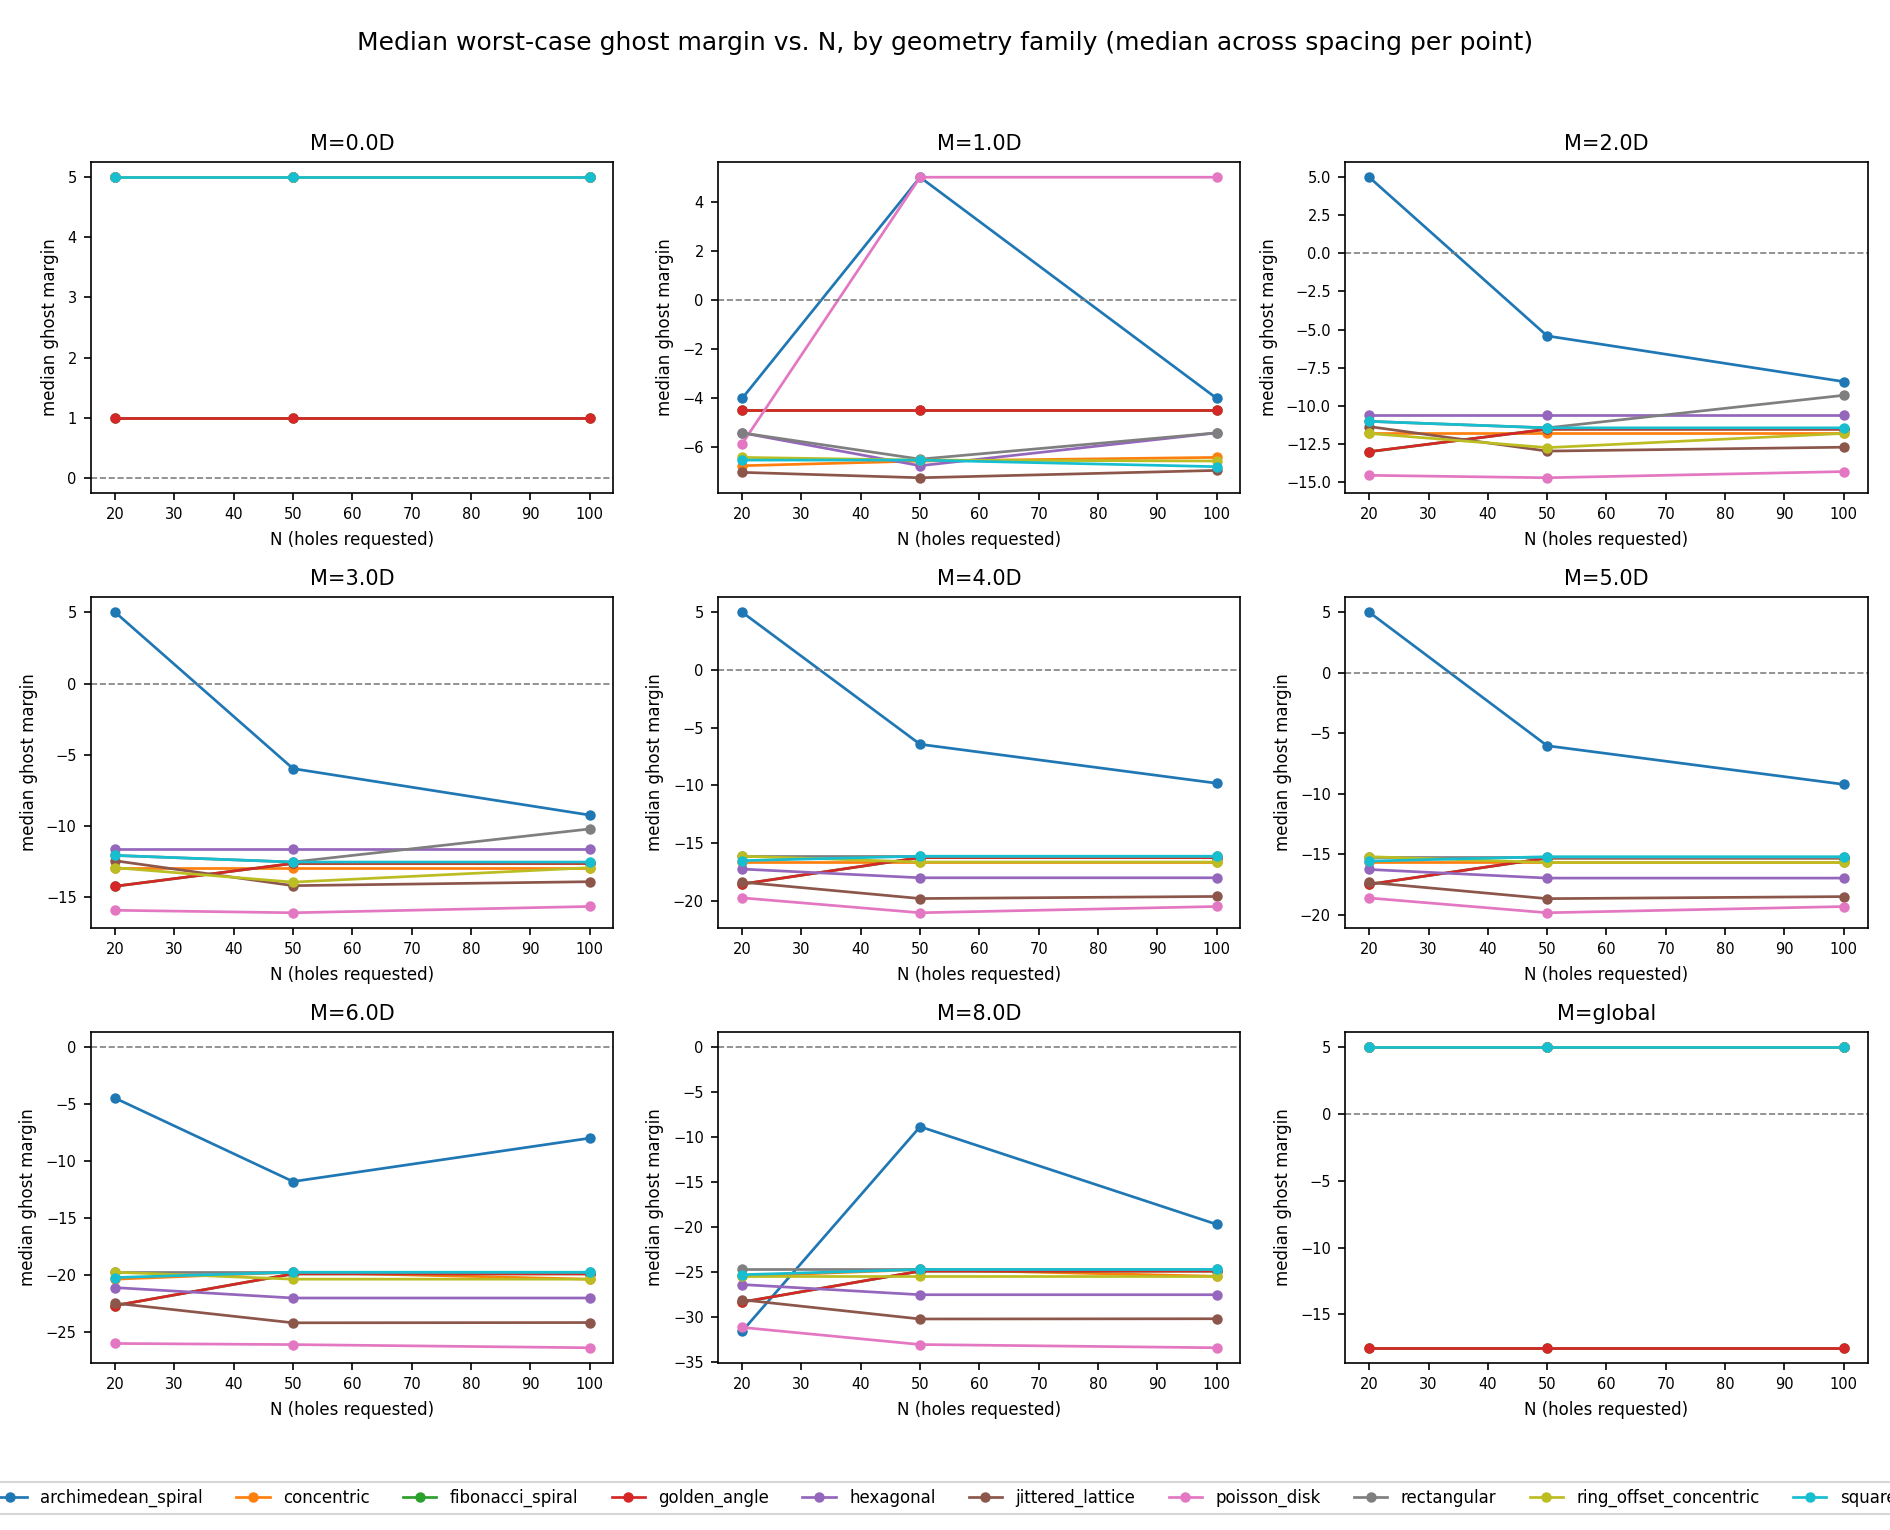
\includegraphics[width=\textwidth]{figures/family_ranking_margin_vs_N.png}
\caption{Median worst-case ghost margin vs.\ $N$ (holes requested), all 11 geometry
families, every $M$ and the global scope -- the full picture behind the winner table
above. Square (cyan) and, separately, golden\_angle (red) are the only families that
stay non-negative at $M=0$D and global scope; at every other $M$, square is again the
only family that survives with a positive/infinite margin, while most of the
remaining 9 families sit well below the $y=0$ safety line regardless of $N$ --
visual confirmation that Model A's structural-safety requirement is a genuinely
narrow target, not an easy bar most designs clear. Source:
\texttt{array\_data/evaluation\_results/family\_ranking\_margin\_vs\_N.png}, mtime
2026-09-13 00:37 (pre-generated by this project's own \texttt{family\_ranking}
analysis, not produced for this paper).}
\label{fig:family-ranking-margin}
\end{figure}
